\documentclass{article}

% Packages required to support encoding
\usepackage{ucs}
\usepackage[utf8x]{inputenc}
\usepackage{graphicx} 
% Packages required by code

% Packages always used
\usepackage{listings}
\usepackage{hyperref}
\usepackage{xspace}
\usepackage[usenames,dvipsnames]{color}
\hypersetup{colorlinks=true,urlcolor=blue}


\usepackage[framed,numbered,autolinebreaks,useliterate] {mcode}


\usepackage{geometry}
\geometry{letterpaper,textwidth=350pt,textheight=680pt,tmargin=60pt,
            left=72pt,footskip=24pt,headsep=18pt,headheight=14pt}
\usepackage{amsmath}
\usepackage{amssymb}
\usepackage{textcase}
\usepackage{soul}

\newcommand{\mat}[1]{\boldsymbol{#1}}\renewcommand{\vec}[1]{\boldsymbol{\mathrm{#1}}}
\newcommand{\vecalt}[1]{\boldsymbol{#1}}

\newcommand{\conj}[1]{\overline{#1}}

\newcommand{\normof}[1]{\|#1\|}
\newcommand{\onormof}[2]{\|#1\|_{#2}}

\newcommand{\itr}[2]{#1^{(#2)}}
\newcommand{\itn}[1]{^{(#1)}}

\newcommand{\eps}{\varepsilon}
\newcommand{\kron}{\otimes}

\DeclareMathOperator{\diag}{diag}
\DeclareMathOperator{\trace}{trace}
\DeclareMathOperator{\tvec}{vec}

\newcommand{\prob}{\mathbb{P}}
\newcommand{\probof}[1]{\prob\left\{ #1 \right\}}

\newcommand{\pmat}[1]{\begin{pmatrix} #1 \end{pmatrix}}
\newcommand{\bmat}[1]{\begin{bmatrix} #1 \end{bmatrix}}
\newcommand{\spmat}[1]{\left(\begin{smallmatrix} #1 \end{smallmatrix}\right)}
\newcommand{\sbmat}[1]{\left[\begin{smallmatrix} #1 \end{smallmatrix}\right]}

\newcommand{\RR}{\mathbb{R}}
\newcommand{\CC}{\mathbb{C}}

\providecommand{\eye}{\mat{I}}
\providecommand{\mA}{\ensuremath{\mat{A}}}
\providecommand{\mB}{\ensuremath{\mat{B}}}
\providecommand{\mC}{\ensuremath{\mat{C}}}
\providecommand{\mD}{\ensuremath{\mat{D}}}
\providecommand{\mE}{\ensuremath{\mat{E}}}
\providecommand{\mF}{\ensuremath{\mat{F}}}
\providecommand{\mG}{\ensuremath{\mat{G}}}
\providecommand{\mH}{\ensuremath{\mat{H}}}
\providecommand{\mI}{\ensuremath{\mat{I}}}
\providecommand{\mJ}{\ensuremath{\mat{J}}}
\providecommand{\mK}{\ensuremath{\mat{K}}}
\providecommand{\mL}{\ensuremath{\mat{L}}}
\providecommand{\mM}{\ensuremath{\mat{M}}}
\providecommand{\mN}{\ensuremath{\mat{N}}}
\providecommand{\mO}{\ensuremath{\mat{O}}}
\providecommand{\mP}{\ensuremath{\mat{P}}}
\providecommand{\mQ}{\ensuremath{\mat{Q}}}
\providecommand{\mR}{\ensuremath{\mat{R}}}
\providecommand{\mS}{\ensuremath{\mat{S}}}
\providecommand{\mT}{\ensuremath{\mat{T}}}
\providecommand{\mU}{\ensuremath{\mat{U}}}
\providecommand{\mV}{\ensuremath{\mat{V}}}
\providecommand{\mW}{\ensuremath{\mat{W}}}
\providecommand{\mX}{\ensuremath{\mat{X}}}
\providecommand{\mY}{\ensuremath{\mat{Y}}}
\providecommand{\mZ}{\ensuremath{\mat{Z}}}
\providecommand{\mLambda}{\ensuremath{\mat{\Lambda}}}
\providecommand{\mPbar}{\bar{\mP}}

\providecommand{\ones}{\vec{e}}
\providecommand{\va}{\ensuremath{\vec{a}}}
\providecommand{\vb}{\ensuremath{\vec{b}}}
\providecommand{\vc}{\ensuremath{\vec{c}}}
\providecommand{\vd}{\ensuremath{\vec{d}}}
\providecommand{\ve}{\ensuremath{\vec{e}}}
\providecommand{\vf}{\ensuremath{\vec{f}}}
\providecommand{\vg}{\ensuremath{\vec{g}}}
\providecommand{\vh}{\ensuremath{\vec{h}}}
\providecommand{\vi}{\ensuremath{\vec{i}}}
\providecommand{\vj}{\ensuremath{\vec{j}}}
\providecommand{\vk}{\ensuremath{\vec{k}}}
\providecommand{\vl}{\ensuremath{\vec{l}}}
\providecommand{\vm}{\ensuremath{\vec{l}}}
\providecommand{\vn}{\ensuremath{\vec{n}}}
\providecommand{\vo}{\ensuremath{\vec{o}}}
\providecommand{\vp}{\ensuremath{\vec{p}}}
\providecommand{\vq}{\ensuremath{\vec{q}}}
\providecommand{\vr}{\ensuremath{\vec{r}}}
\providecommand{\vs}{\ensuremath{\vec{s}}}
\providecommand{\vt}{\ensuremath{\vec{t}}}
\providecommand{\vu}{\ensuremath{\vec{u}}}
\providecommand{\vv}{\ensuremath{\vec{v}}}
\providecommand{\vw}{\ensuremath{\vec{w}}}
\providecommand{\vx}{\ensuremath{\vec{x}}}
\providecommand{\vy}{\ensuremath{\vec{y}}}
\providecommand{\vz}{\ensuremath{\vec{z}}}
\providecommand{\vpi}{\ensuremath{\vecalt{\pi}}}

\sodef\allcapsspacing{\upshape}{0.15em}{0.65em}{0.6em}%

\makeatletter
\def\maketitle{%
\par
\hrule height 0.75pt\vspace{1ex}
\par\noindent
\begin{minipage}{0.5\textwidth}
\scshape
purdue university $\cdot$ CS 580 \\
Introduction to the Analysis of Algorithms
\end{minipage}
\begin{minipage}{0.5\textwidth}
\raggedleft
\MakeTextUppercase{\allcapsspacing{\@title}}\\[0.2ex]
\textit{\@author}\\[0.2ex]
\textit{\@date}
\end{minipage}
\par\vspace{1ex}
\hrule height 1pt
\vspace{2ex}
\par
}
\makeatother

\author{Jun Cheng}
\title{Lecture Notes}
% auto generate a title
\AtBeginDocument{\maketitle}


\title{Homework}



\begin{document} 


\subsection*{{Problem 1: }}
\begin{align*} 
y_k=ay_{k-1} + bu_k + v_k\\
(y_k-ay_{k-1}) = bu_k + v_k \\
\end{align*}
where $v_k$ represents white noise. Then we need minimize: \\
\begin{align*} 
\|(y_k-ay_{k-1}-bu_k\| 
\end{align*}


\subsection*{{Problem 2: }}

Using PSO algorithm, we can find the minimizer: \\
\begin{align*}
x_0 & = 0.000279321964182 \\
x_1 & = 0.000193196456243 \\
f(x_0,x_1) & =  2.28836604776e-07
\end{align*}

\begin{figure}[h]
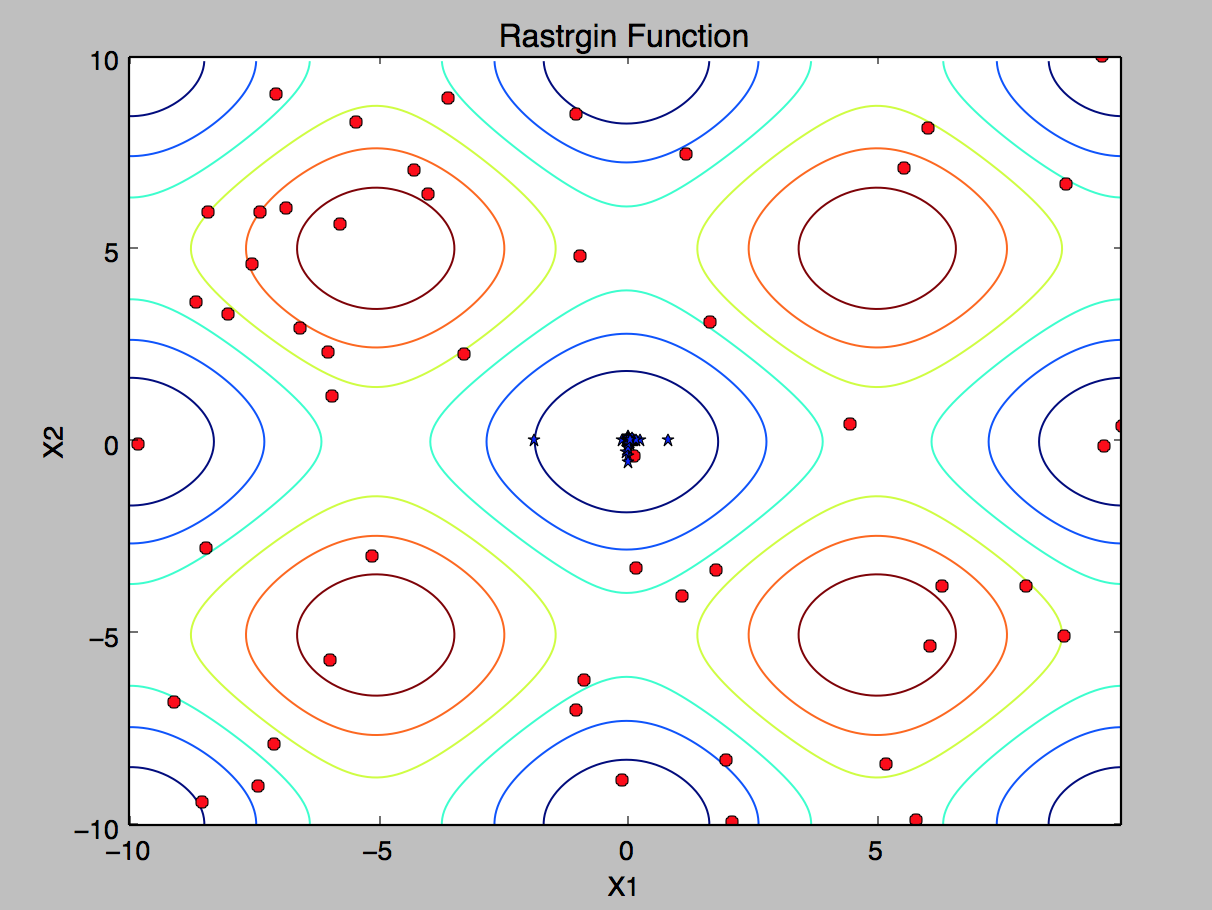
\includegraphics[width=0.7\textwidth]{PSO} 
\centering
\caption{PSO Algorithm (problem 2): circle points are randomly generated 50 initial points. Stars indicate the positions after 50 iterations. }

\end{figure}

\begin{figure}[h]
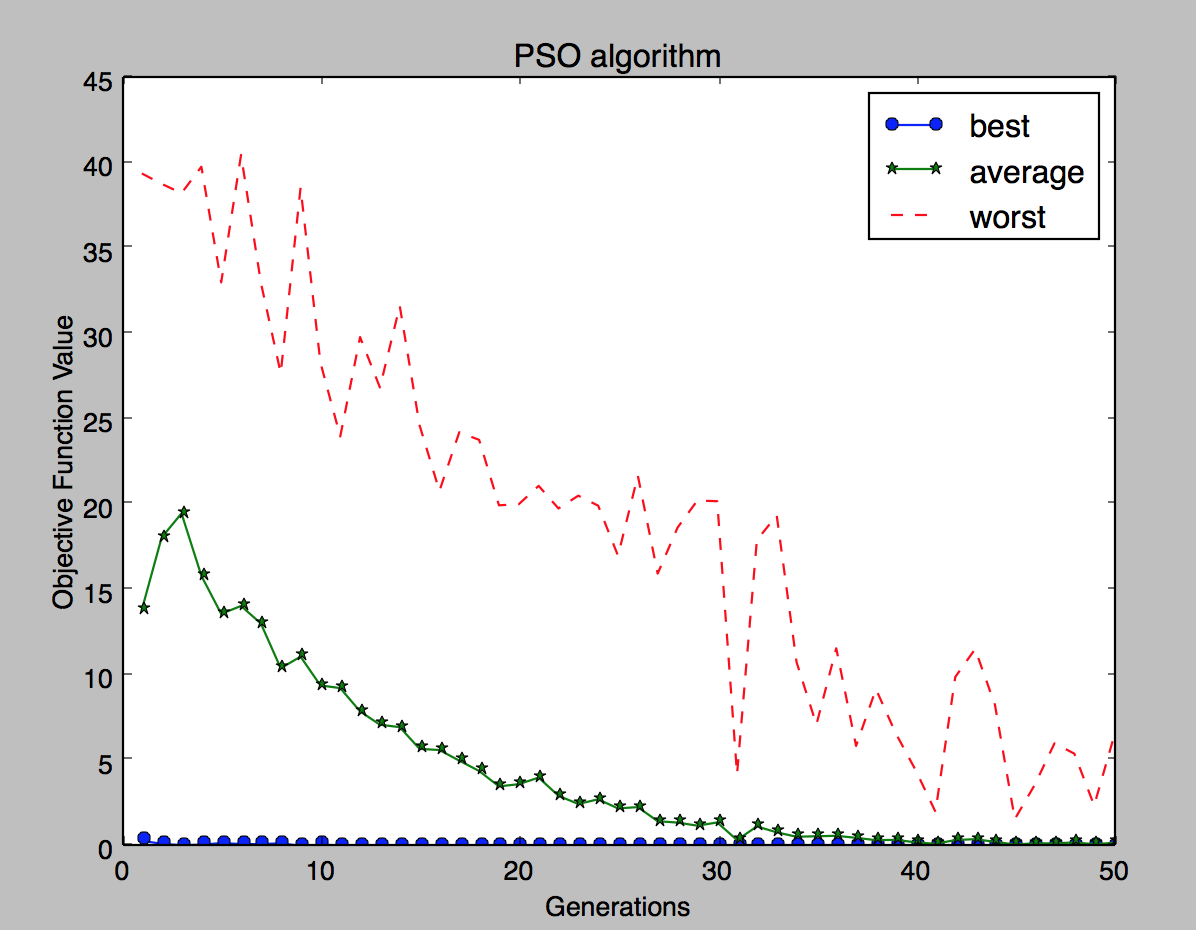
\includegraphics[width=0.7\textwidth]{PSO_min_best} 
\centering
\caption{PSO Algorithm (problem 2): plots of the best, average, and the worst objective function values in the population for 50 generations }

\end{figure}


\subsection*{{Problem 3: }}

Using PSO algorithm, we can find the maximizer: \\
\begin{align*}
x_0 & =  -5.02482780601\\
x_1 & =  5.02524813509\\
f(x_0,x_1) & = -40.5025451078 
\end{align*}
In fact, there are several other global maximizers. PSO method will converge to different global maximizer depending on the initial points which are randomly chosen.   
\begin{figure}[h]
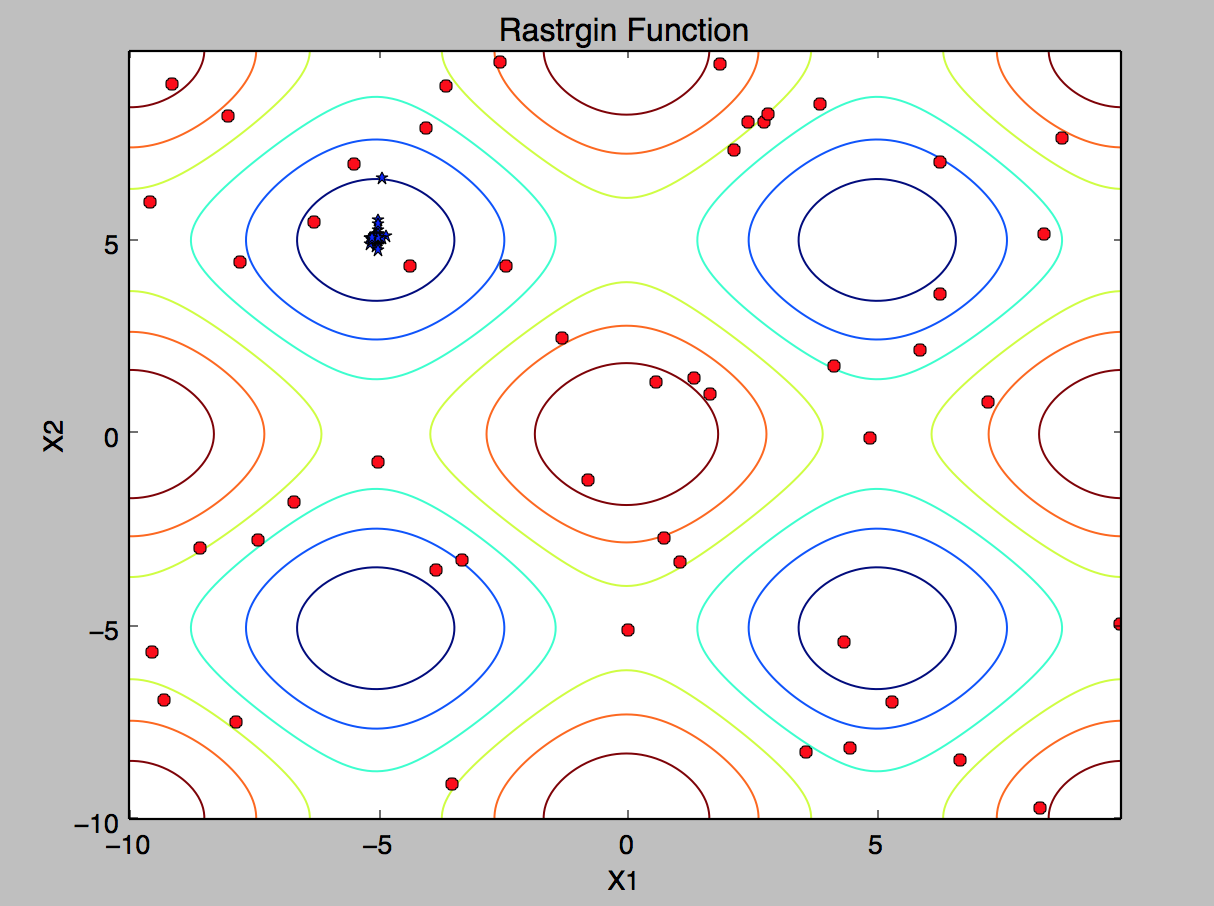
\includegraphics[width=0.7\textwidth]{PSO_max} 
\centering
\caption{PSO Algorithm (problem 3): circle points are randomly generated 50 initial points. Stars indicate the positions after 50 iterations. }

\end{figure}

\begin{figure}[h]
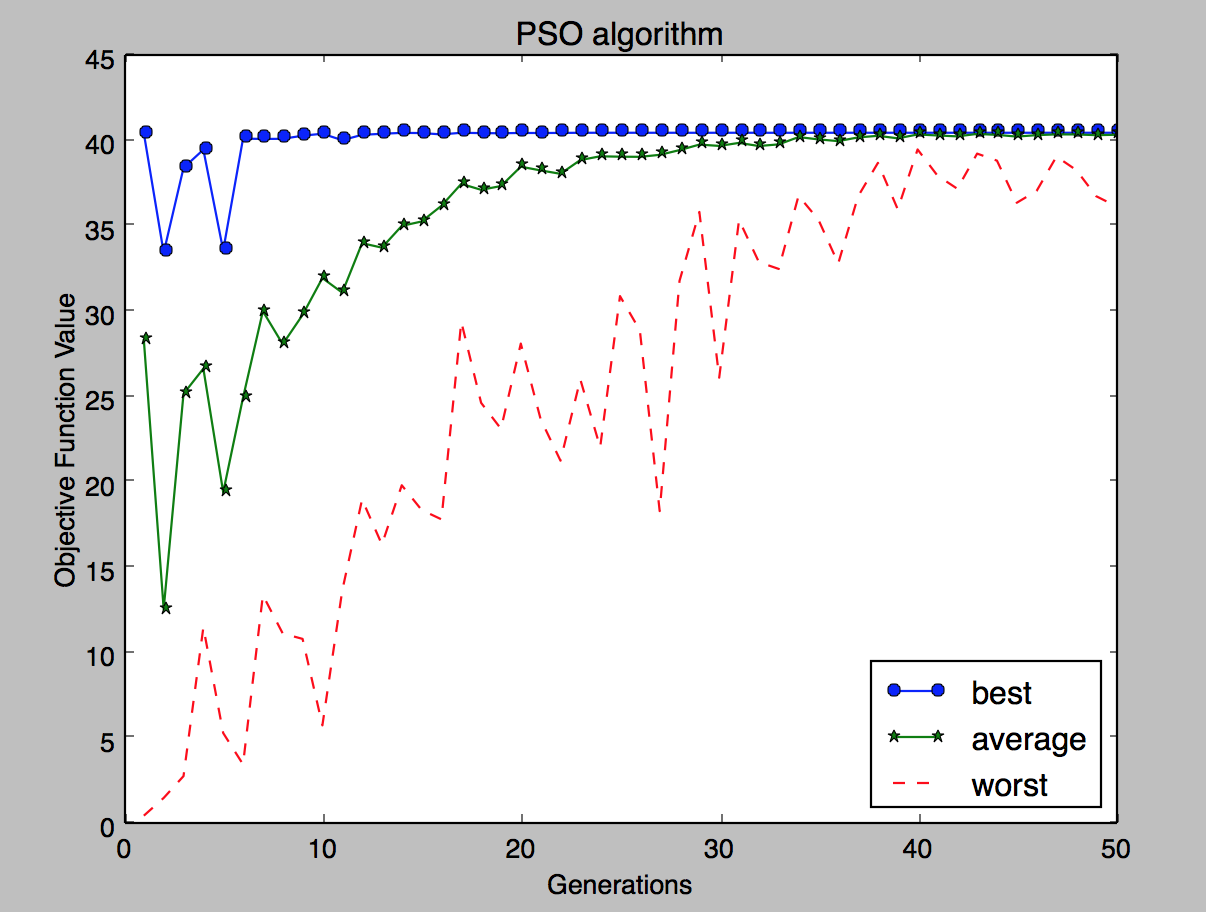
\includegraphics[width=0.7\textwidth]{PSO_max_best} 
\centering
\caption{PSO Algorithm (problem 3): plots of the best, average, and the worst objective function values in the population for 50 generations }

\end{figure}





\subsection*{{Problem 4: }}

Population size:  50  \\
Number of iterations:  50 \\ 
For canonical number genetic algorithm, the minimizer is: \\
\begin{align*}
x_1 & = 0.0408935546875 \\
x_2 & = 0.0390625  \\
f(x_1,x_2)  & = 0.00634456702034
\end{align*}

For real number genetic algorithm, the minimizer is : \\
\begin{align*} 
x_1 & = 0.018313265874 \\
x_2 & = 0.0286761643909 \\
f(x_1, x_2) & = 0.00229673023909
\end{align*} 

\begin{figure} [h]
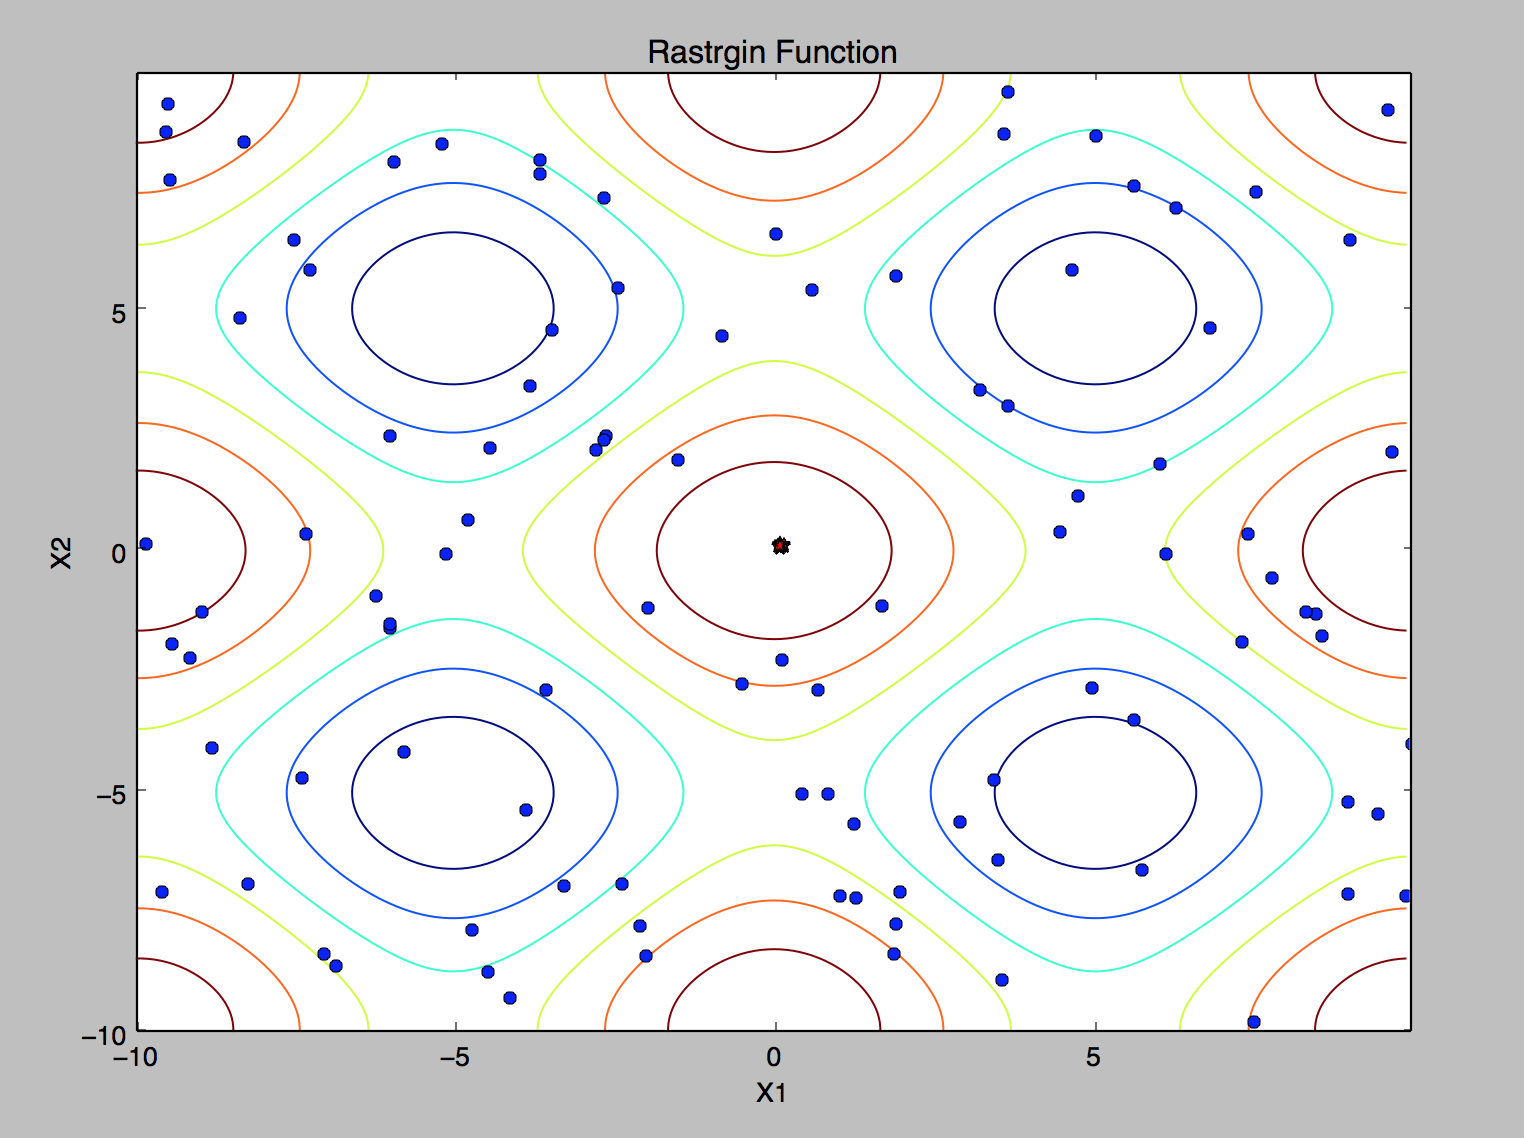
\includegraphics[width=0.7\textwidth]{GA_canonical}
\centering
\caption{Canonical Genetic Algorithm (problem 4): circle points are randomly generated 50 initial points. Stars indicate the positions after 50 iterations. }

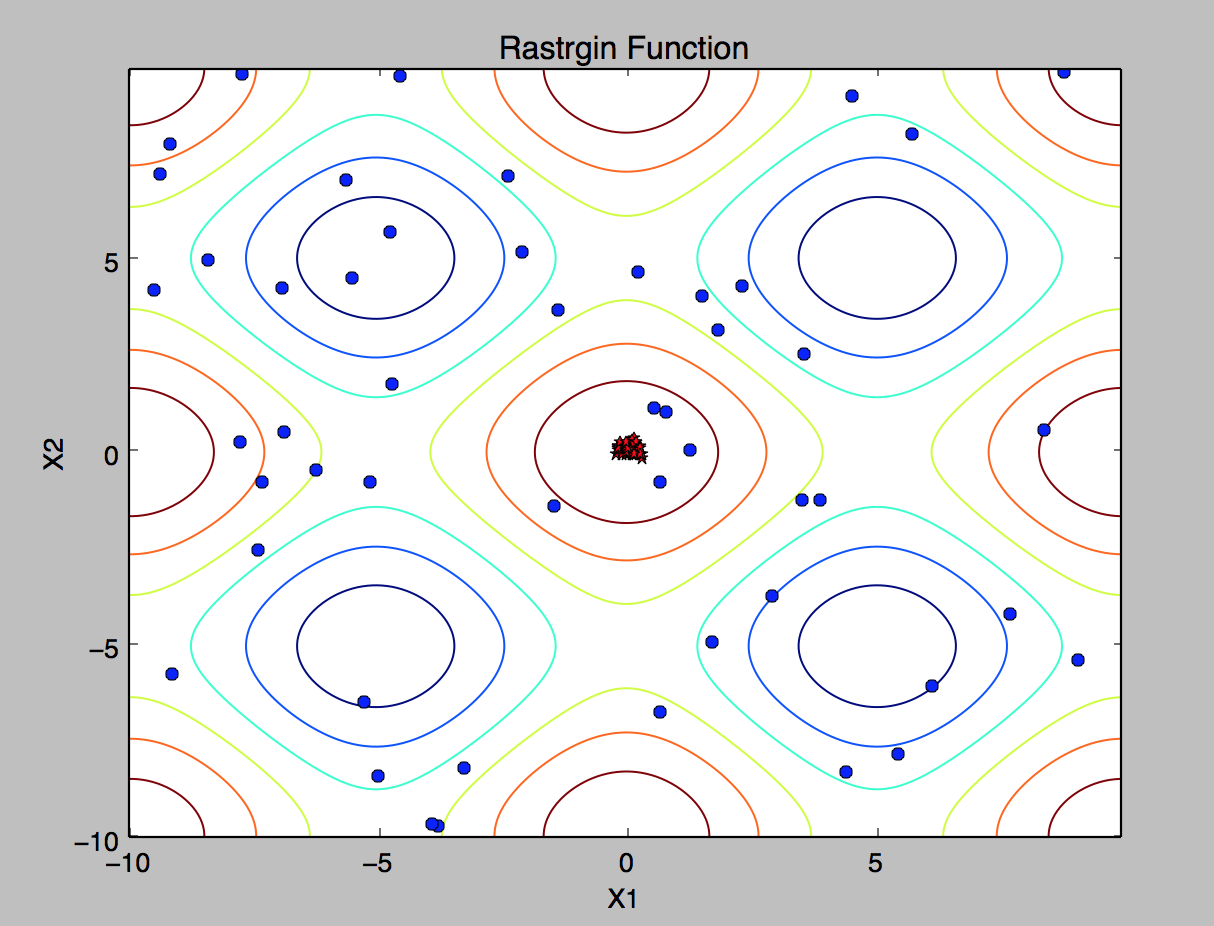
\includegraphics[width=0.7\textwidth]{GA_real_number}
\centering
\caption{Real Number Genetic Algorithm (problem 4): circle points are randomly generated 50 initial points. Stars indicate the positions after 50 iterations. }

\end{figure}

\begin{figure}[h]
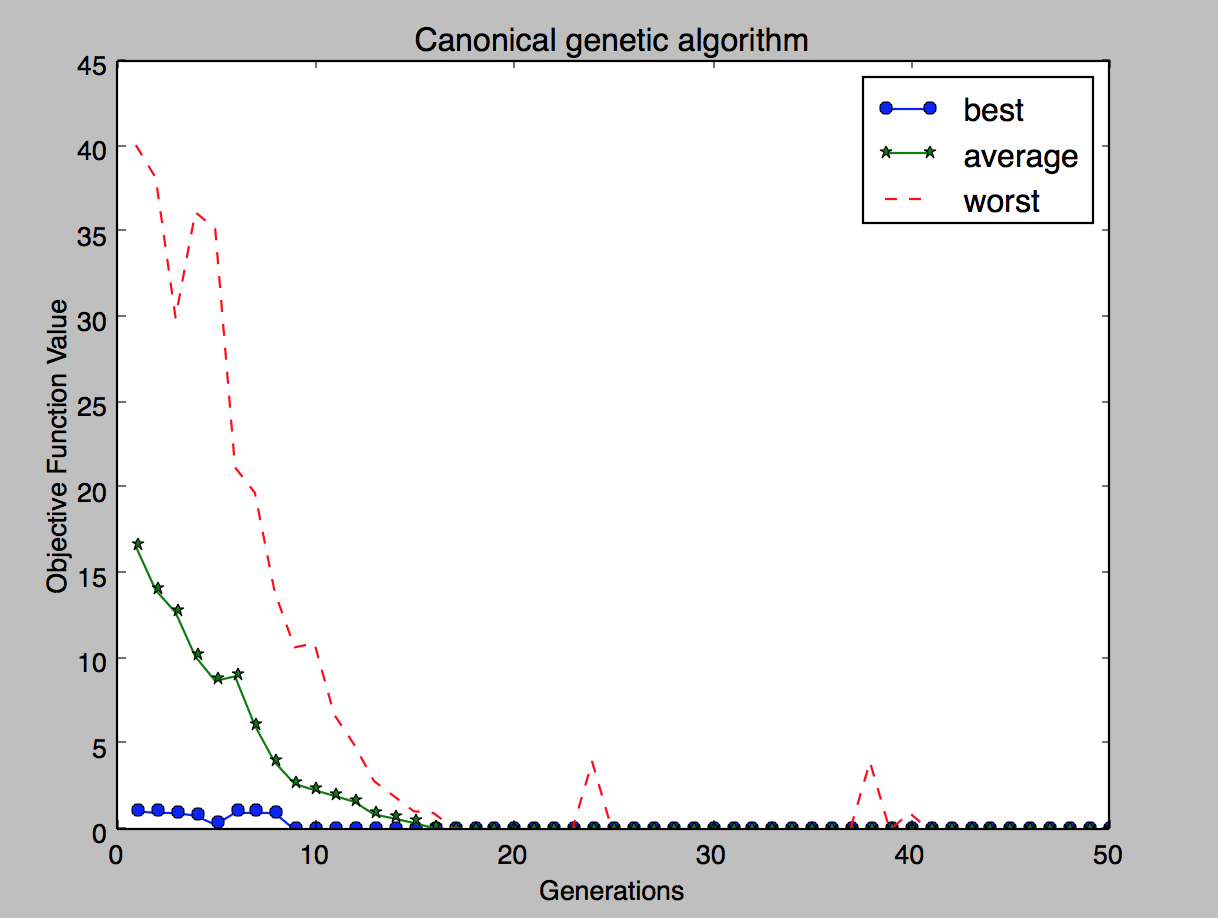
\includegraphics[width=0.7\textwidth]{Canonical_GA_best_plot}
\centering
\caption{Canonical Genetic Algorithm (problem 4): plots of the best, average, and the worst objective function values in the population for 50 generations}


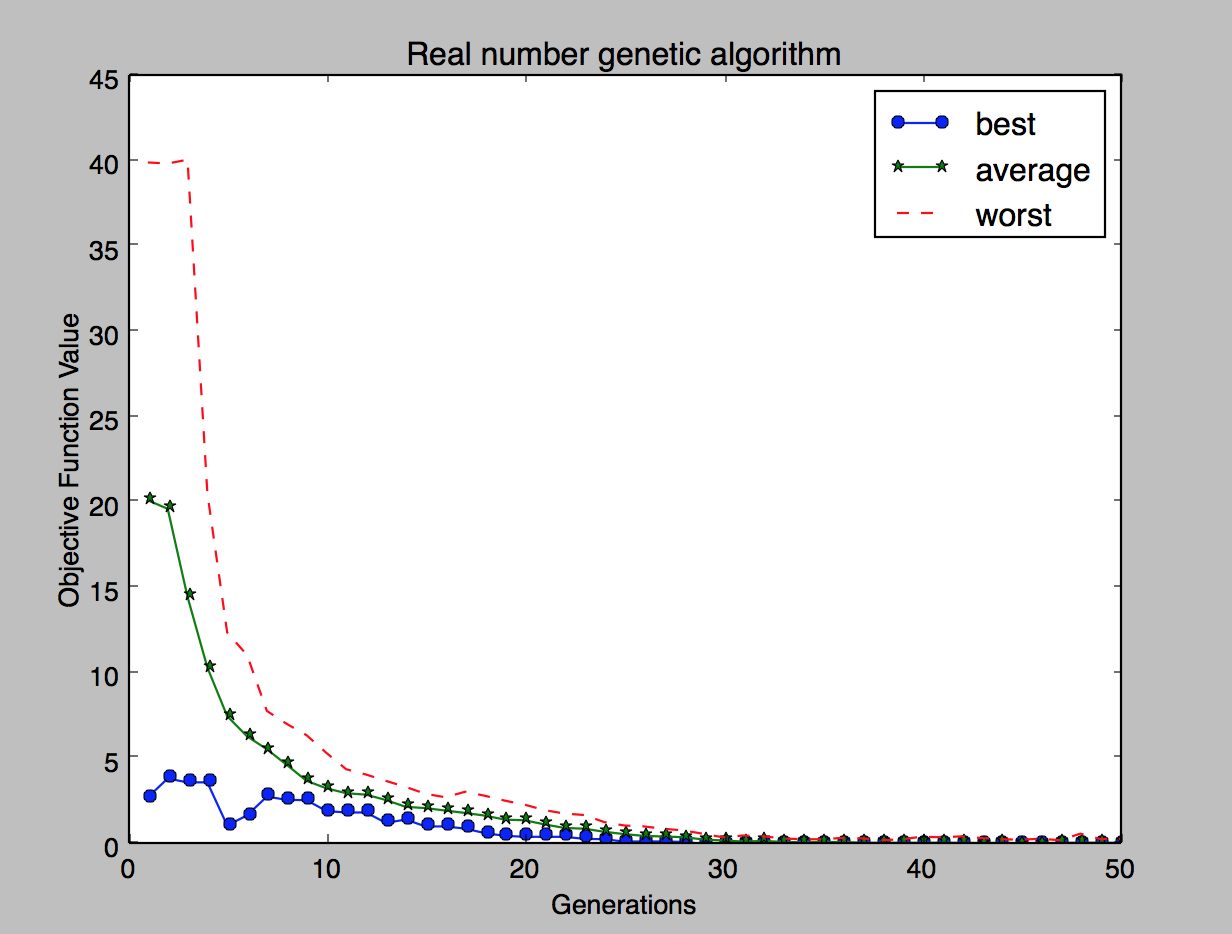
\includegraphics[width=0.7\textwidth]{Real_number_GA}
\centering
\caption{Real Number Genetic Algorithm (problem 4): plots of the best, average, and the worst objective function values in the population for 50 generations}
\end{figure}


\subsection*{{Problem 5: }}

The shortest path is shown in Figure \ref{fig:tsp1}, and the shortest distance is : $37.7222579198$

\begin{figure}[h]
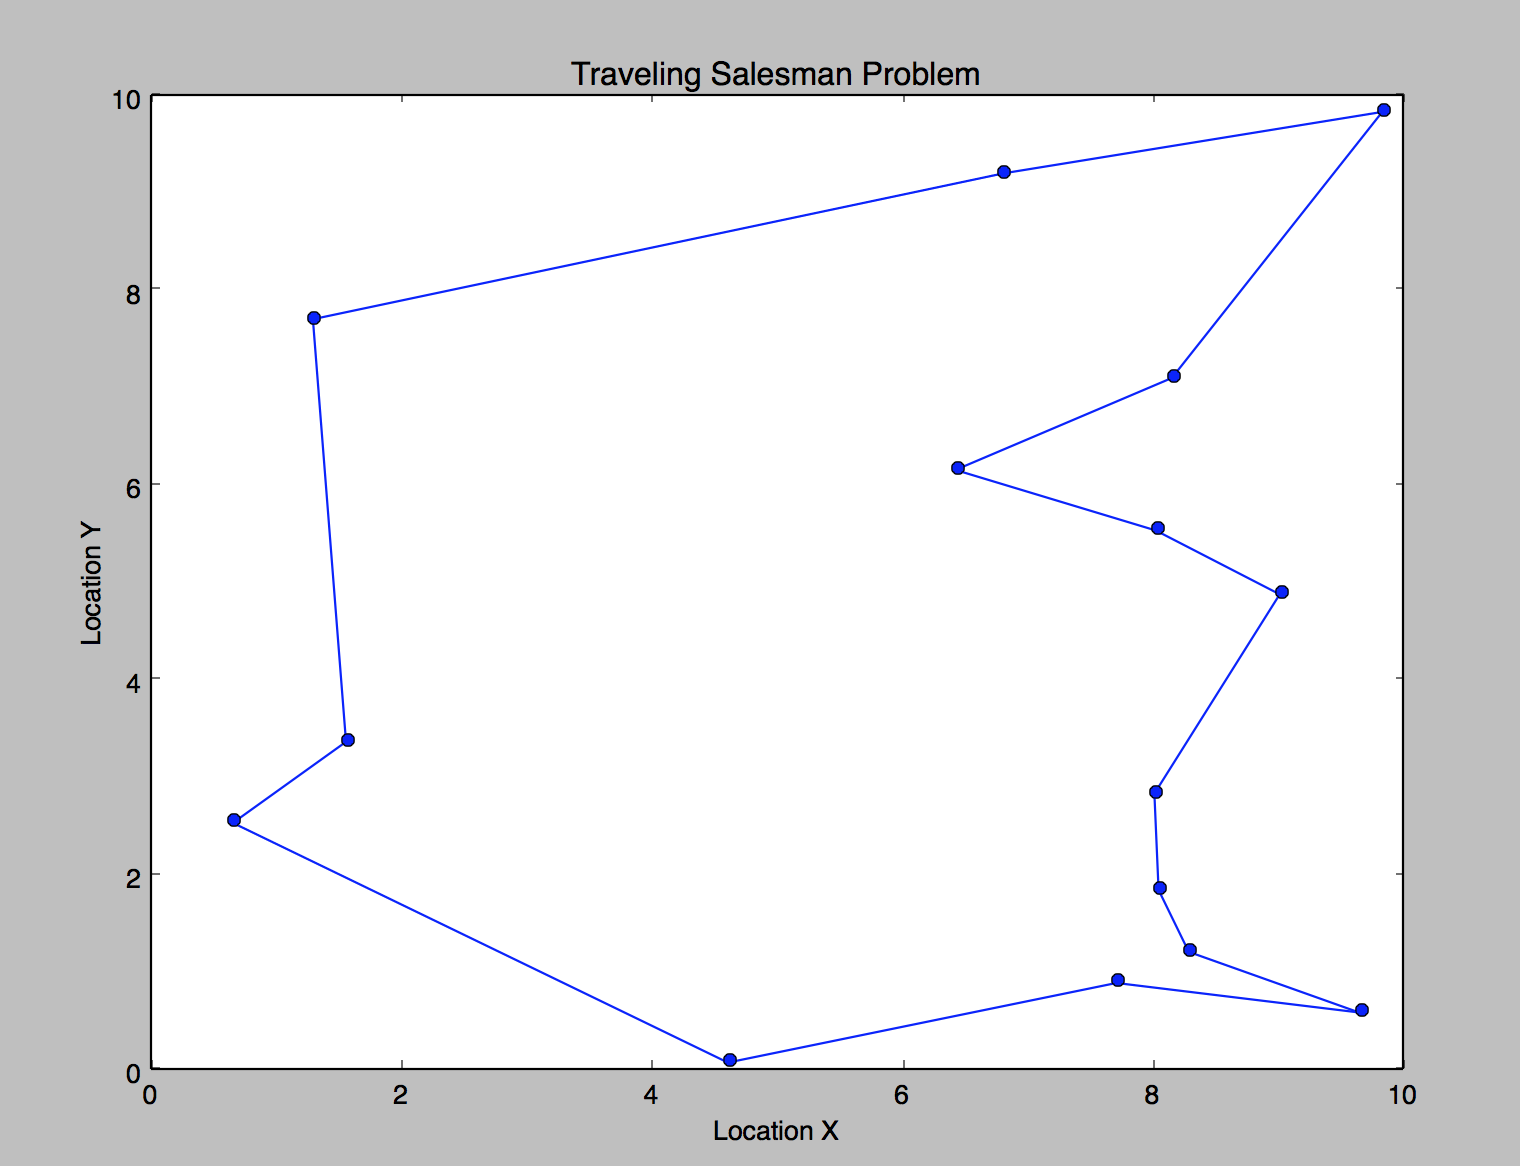
\includegraphics[width=0.7\textwidth]{Traveling_salesman_path}
\centering
\caption{Traveling salesman problem (problem 5): plots of the shortest distance path}
\label{fig:tsp1}

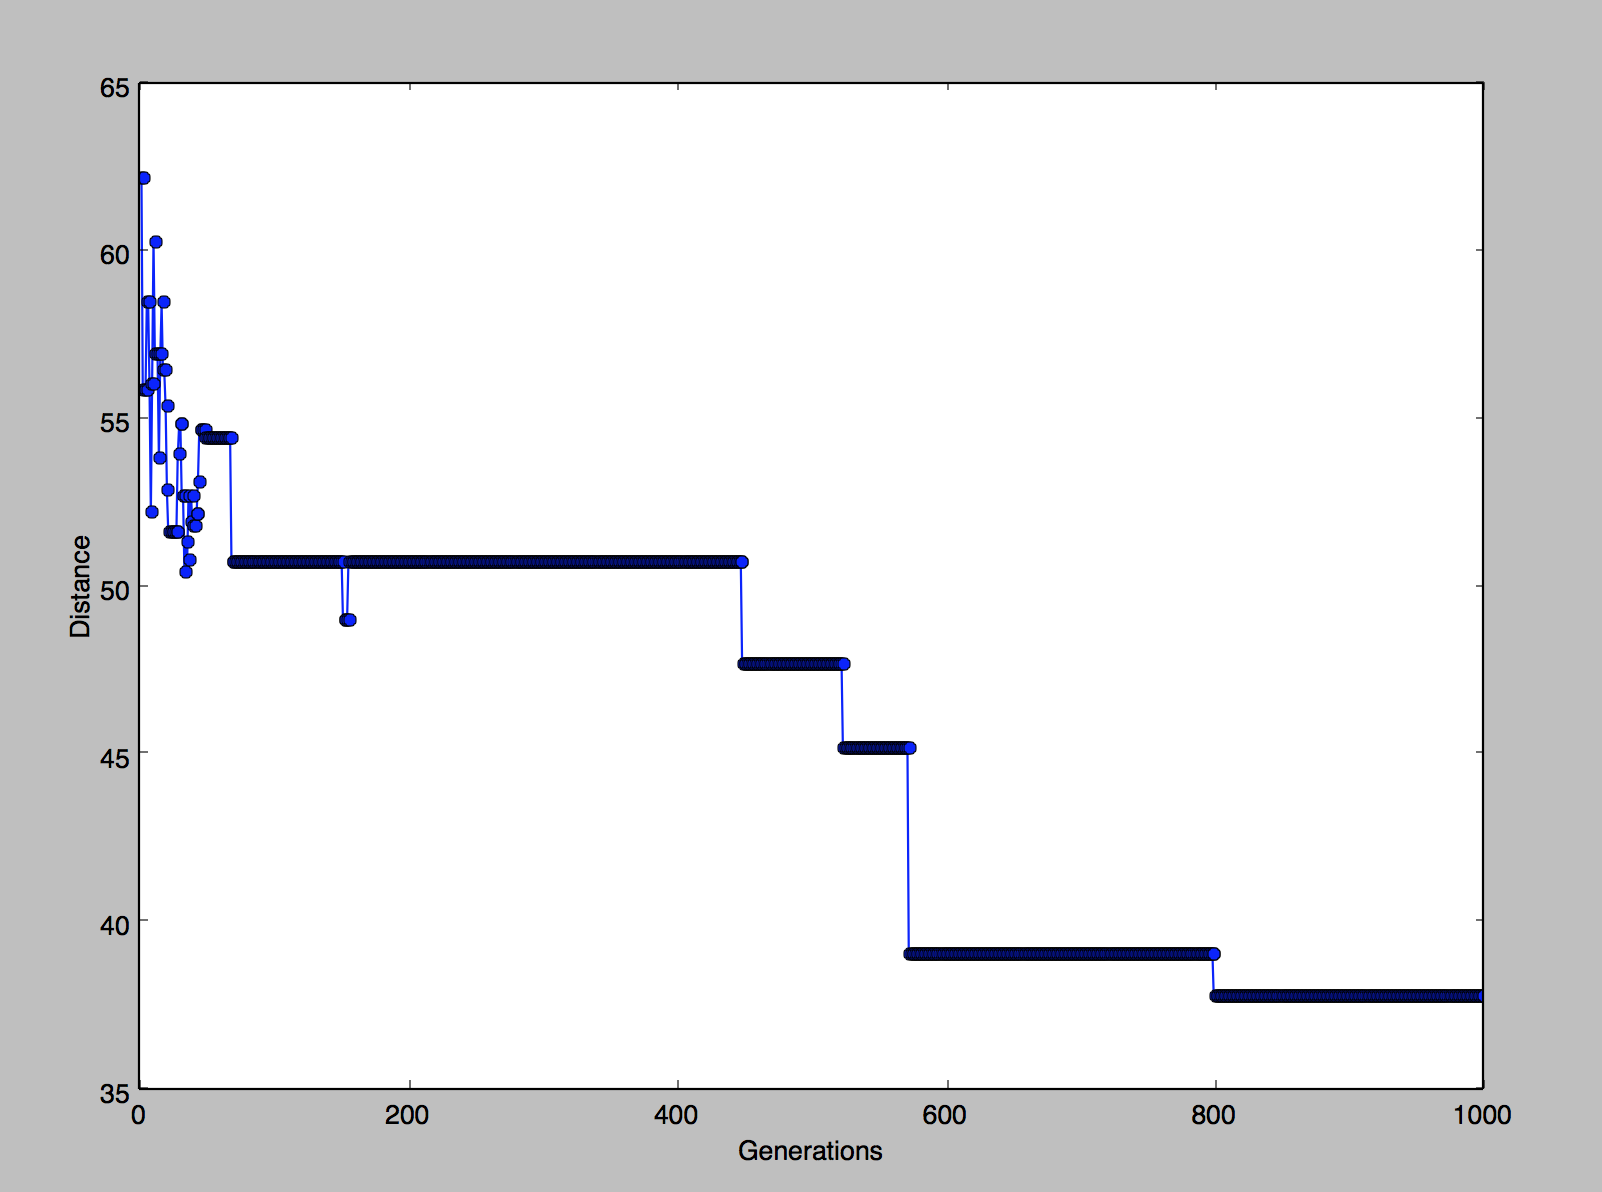
\includegraphics[width=0.7\textwidth]{Distance_vs_generation}
\label{fig:tsp2}
\centering
\caption{Traveling salesman problem (problem 5): plots of the shortest distance for different combinations of the population for 1000 generations}

\end{figure}

\subsection*{{Problem 6: }}


Matlab code for Problem 6: \\
\begin{lstlisting} 
f = [7  10  14  8   7   11  12  6   5   8   15  9   ]; 
A = [];
b = [];
Aeq = [1    1   1   1	0   0   0   0   0   0   0   0; 
       0    0   0   0    1    1   1   1    0   0   0   0 ; 
       0    0   0   0    0    0   0   0    1    1   1   1; 
       1    0   0   0    1    0   0   0    1    0   0   0; 
       0    1   0   0    0    1   0   0    0    1   0   0 ; 
       0    0   1   0    0    0   1   0    0    0   1   0 ;   
       0    0   0   1    0    0   0   1    0    0   0   1  ]; 
beq = [30   40  30  20  20  25  35];
lb = [0, 0, 0, 0, 0, 0, 0, 0, 0, 0, 0, 0]; 
ub = [] ; 
x = linprog(f, A, b, Aeq, beq, lb, ub) 
\end{lstlisting}
The output: 
\begin{lstlisting}
x =

    4.8834
    5.1166
    8.7304
   11.2696
    0.0000
    0.0000
   16.2696
   23.7304
   15.1166
   14.8834
    0.0000
    0.0000
\end{lstlisting}



\end{document}
